\section{Exploración del tamaño de población}

\begin{table}[]
    \centering
    \begin{tabular}{|c|c|c|c|c|c|}
        \hline
        \textbf{Config.} & \textbf{\begin{tabular}[c]{@{}c@{}}Tmñ.\\ Población\end{tabular}} & \textbf{\begin{tabular}[c]{@{}c@{}}Mediana \\ mejor valor \\ de fitness\end{tabular}} & \textbf{\begin{tabular}[c]{@{}c@{}}Mediana \\ \# ejecuciones \\ de f\end{tabular}} & \textbf{\begin{tabular}[c]{@{}c@{}}$\sigma$\\ mejor valor\\ de fitness\end{tabular}} & \textbf{\begin{tabular}[c]{@{}c@{}}$\sigma$\\ \# ejecuciones \\ de f\end{tabular}} \\ \hline
        4  [\ref{subsect:config_file_4}]                & 100                                                               & 7.00                                                                                  & 7852.0                                                                             & 11.98                                                                         & 2045.87                                                                     \\ \hline
        7  [\ref{subsect:config_file_7}]                & 150                                                               & 0.27                                                                                  & 9010.0                                                                             & 15.10                                                                         & 2536.42                                                                     \\ \hline
        8  [\ref{subsect:config_file_8}]                & 300                                                               & -18.06                                                                                & 23496.0                                                                            & 10.20                                                                         & 6406.70                                                                     \\ \hline
        9  [\ref{subsect:config_file_9}]                & 500                                                               & -26.11                                                                                & 37087.0                                                                            & 5.61                                                                          & 8492.77                                                                     \\ \hline
        10 [\ref{subsect:config_file_10}]               & 1000                                                              & -33.53                                                                                & 75539.5                                                                            & 5.63                                                                          & 21178.32                                                                    \\ \hline
    \end{tabular}
    \caption{Resultados exploración inicial para diferentes tamaños de población}
    \label{tab:base_population}
\end{table}

El objetivo de esta sección es obtener una población inicial base para las próximas exploraciones. Dejaremos fija la dimensión del cromosoma a 10 y
ejecutaremos cada fichero de configuración 15 veces. Se ha escogido esta dimensión porque ha alcanzado una solución 
relativamente buena en el experimento anterior. Las soluciones de esta exploración se encuentran en la Tabla \ref{tab:base_population}. 
En esta nueva exploración se han probado los tamaños de población: 100, 150, 300, 500, 1000, indicados en la Tabla \ref{tab:base_population}
como \textit{Tmñ. poblacion}. En la Figura \ref{fig:population_size_variation} se vuelve a ver cómo el mayor descenso del valor del fitness se produce
entre la generación 0 y la 20. La población con tamaño 1000 (Config 10 en Tabla \ref{tab:base_population}) es la que tiene
un mayor descenso pasada la generación 20. 

\begin{figure}[]
	\centering	
	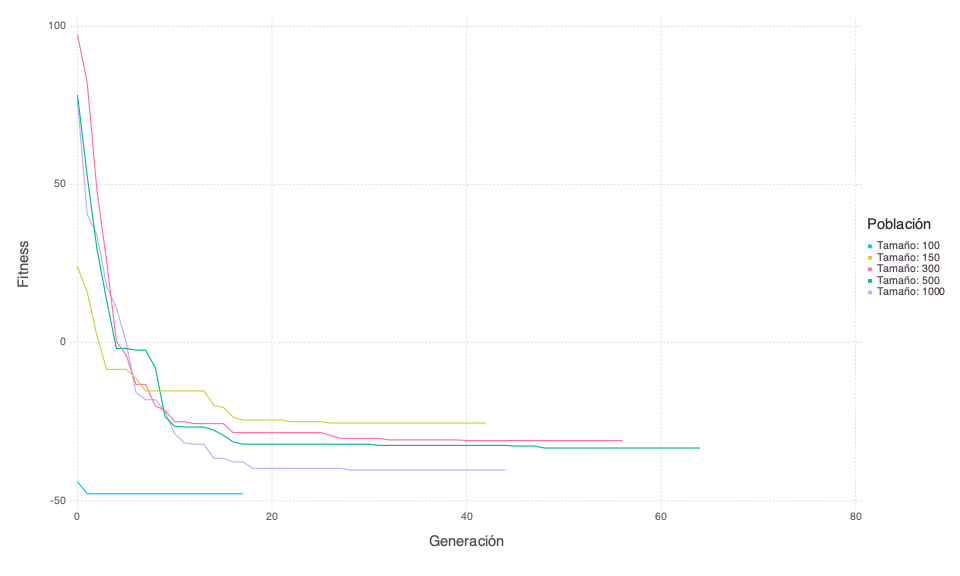
\includegraphics[scale=0.5]{../data/Plots/population_size_variation.png}
	\caption{ Ejecuciones variando el tamaño de la población }
    \label{fig:population_size_variation}
\end{figure}

En la Figura \ref{fig:population_size_box_plots}, se ve que la configuración 4 [\ref{subsect:config_file_4}] es la que alcanza un valor más pequeño de fitness.
Sin embargo mirando la Tabla \ref{tab:base_population} es la configuración 10 [\ref{subsect:config_file_10}] la que tiene mejor mediana para el valor del 
fitness, y además menor desviación típica, por lo que en general se mueve por solciones relativamente buenas.

\begin{figure}[]
	\centering	
	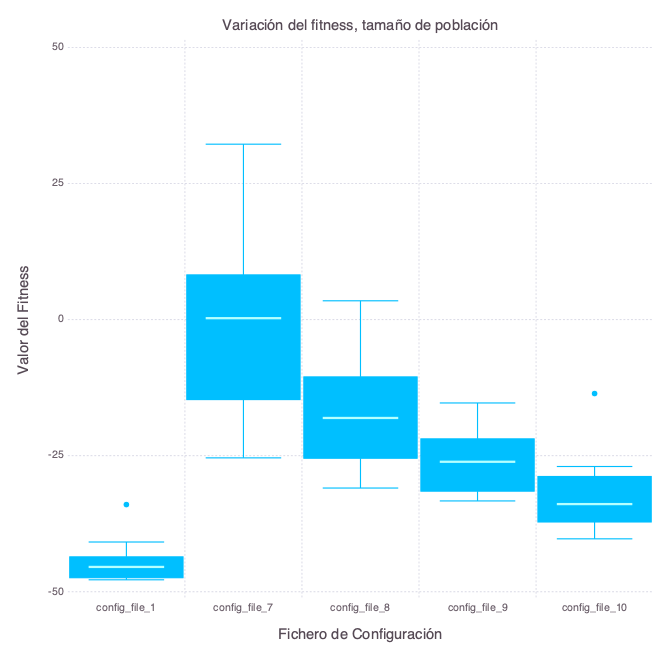
\includegraphics[scale=0.5]{../data/Plots/Rastrigin_box_plots_p_size.png}
	\caption{ Diversidad en la ejecución variando el tamaño de población }
    \label{fig:population_size_box_plots}
\end{figure}


El objetivo de esta exploración era sacar una población inicial en la que basar el resto de experimentos. Por tanto atendiendo al que tiene mejor mediana,
usaremos la configuración 10 [\ref{subsect:config_file_10}] para las siguientes exploraciones.